\documentclass{article}
\usepackage{amsmath,amsthm,amsfonts}
\usepackage{graphicx}
% \newtheorem{theorem}{Theorem}
\newtheorem{theorem}{Theorem}[section]
\newtheorem{corollary}{Corollary}[section]

\newcommand{\R}{\mathbb{R}}
% cv for column vector
\newcommand{\cv}[2]{\begin{bmatrix}
#1\\
#2\\
\end{bmatrix}
}

\title{Lecture 2}
\author{Dark Lord}

\begin{document}
\maketitle

\section*{Equations}


\begin{equation}
    \label{limit}
    e = \lim_{t \to \infty} {\left( 1+t \right)}^t
\end{equation}


\begin{align}
    % \label{limit2}
    e  &= \lim_{t \to \infty} {\left( 1+t \right)}^t\\
    \text{Like and Subscribe} &= \lim_{t \to \infty} {\left( 1+t \right)}^t
\end{align}

\begin{equation}
\begin{split}
    % \label{limit3}
    e &= \lim_{t \to \infty} {\left( 1+t \right)}^t \\
    \text{Like and Subscribe} &= \lim_{t \to \infty} {\left( 1+t \right)}^t
\end{split}
\end{equation}
% Equation 1 is very cool
Equation~\ref{limit} is very cool


 % for long equations which do not fit in one line

\begin{multline}
    e \approx 1+x+ \frac{x^2}{2!}+ \frac{x^3}{3!} + \frac{x^4}{4!} + \frac{x^5}{5!}\\    
    +\frac{x^6}{6!} + \frac{x^7}{7!} + \frac{x^8}{8!}
\end{multline}


\newpage

\section{Tables}



\begin{table}
\caption{NIFTY table}\label{niftytable}
\begin{center}
    \begin{tabular}{|c|r|}
        \hline
        1 & 2 \\ \hline
        3 & 400000000000000 \\ \hline
    \end{tabular}
\end{center}
\end{table}

I like table no~\ref{niftytable}

\newpage


% \section{Graphics}

\begin{figure}
    \centering
    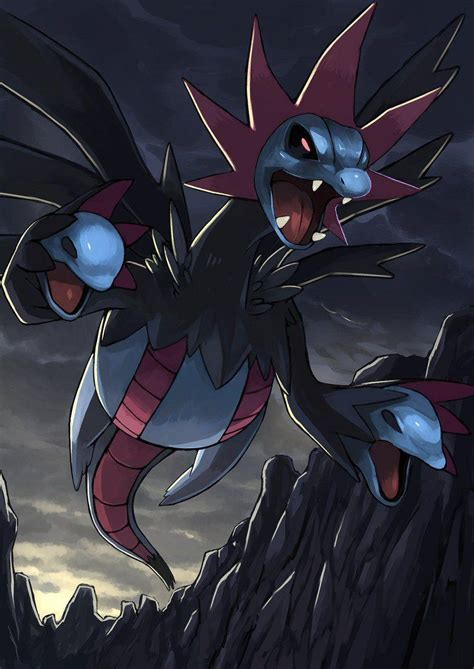
\includegraphics[width=\textwidth]{img1}
    \caption{Hydreigon}\label{hydreigon}

\end{figure}


\newpage
\section{New Theorem command}

\begin{theorem}[YouTube]
You should like and subscribe
\end{theorem}
\begin{proof}
Left to the interested subscriber
\end{proof}
\begin{theorem}
You should ring the notification bell
\end{theorem}

\begin{corollary}
Check out overleaf as well
\end{corollary}


\section{Macros}


The real number $\mathbb{R}$
% mathbb requires amsfonts

The real number $\R$

\vspace{20pt}

% bmatrix bracket matrix
Bracket matrix \textbf{traditional way}
\[
    \begin{bmatrix}
        a\\
        b\\
    \end{bmatrix}
\]

Bracket matrix \textbf{\textit{issuing newcommand}}
\[
    \cv{c}{d}
\]

\end{document}
